%! Author = kaliw
%! Date = 12/10/2019

% Convolutional Net

Our most evolved net Charizard, was created using a convolutional neural network.
The network architecture we use is:
\begin{enumerate}
    \item Convolution 32@2x2
    \item Batch Normalization
    \item ReLU
    \item Convolution 64@2x2
    \item Batch Normalization
    \item ReLU
    \item Convolution 32@2x2
    \item Fully Connected 512x1
    \item Fully Connected 128x1
    \item Fully Connected 3x1
    \item Softmax
\end{enumerate}
We trained over 20 epochs, and used an Adam optimizer with a learning rate of 0.0001, $\beta_1$ of 0.9 and $\beta_2$ of 0.999.
These are the results of the training runs
\begin{figure}[h!]
	\centering
	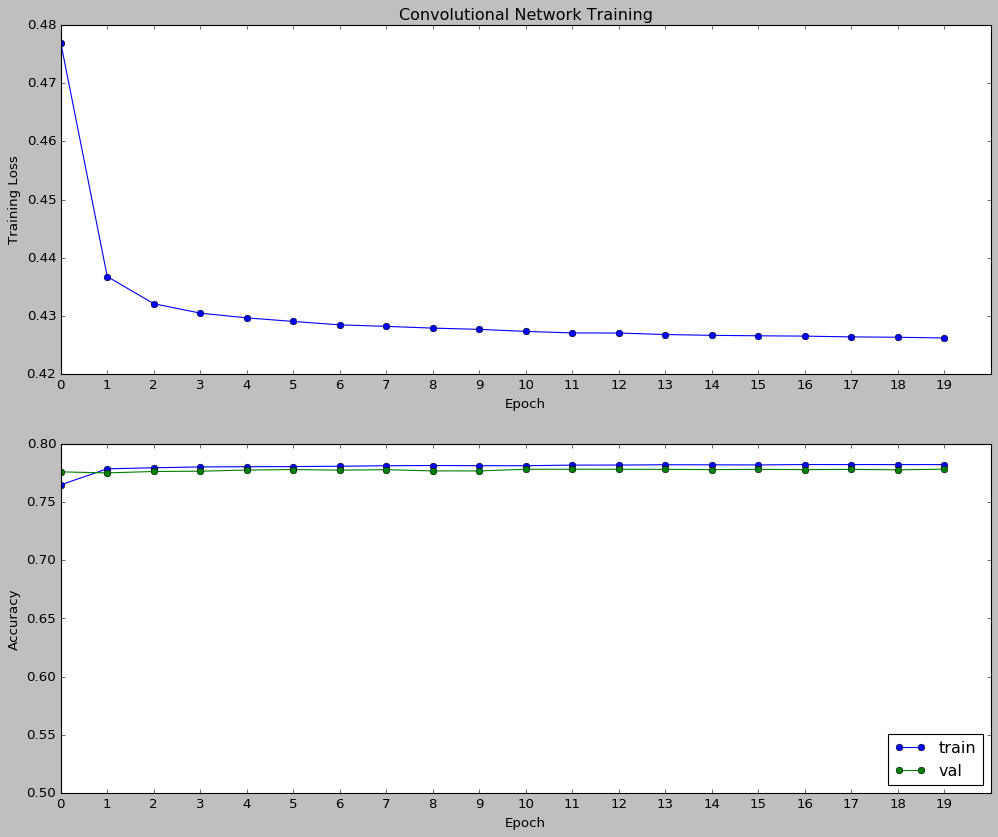
\includegraphics[width=10cm, height=7cm]{convolutional-net-training.png}
	\caption{Top: Training loss over 20 epochs. Bottom: Training accuracy against validation accuracy over 20 epochs}
	\label{fig:conv_net}
\end{figure}

